\begin{figure}[H]
    \centering
    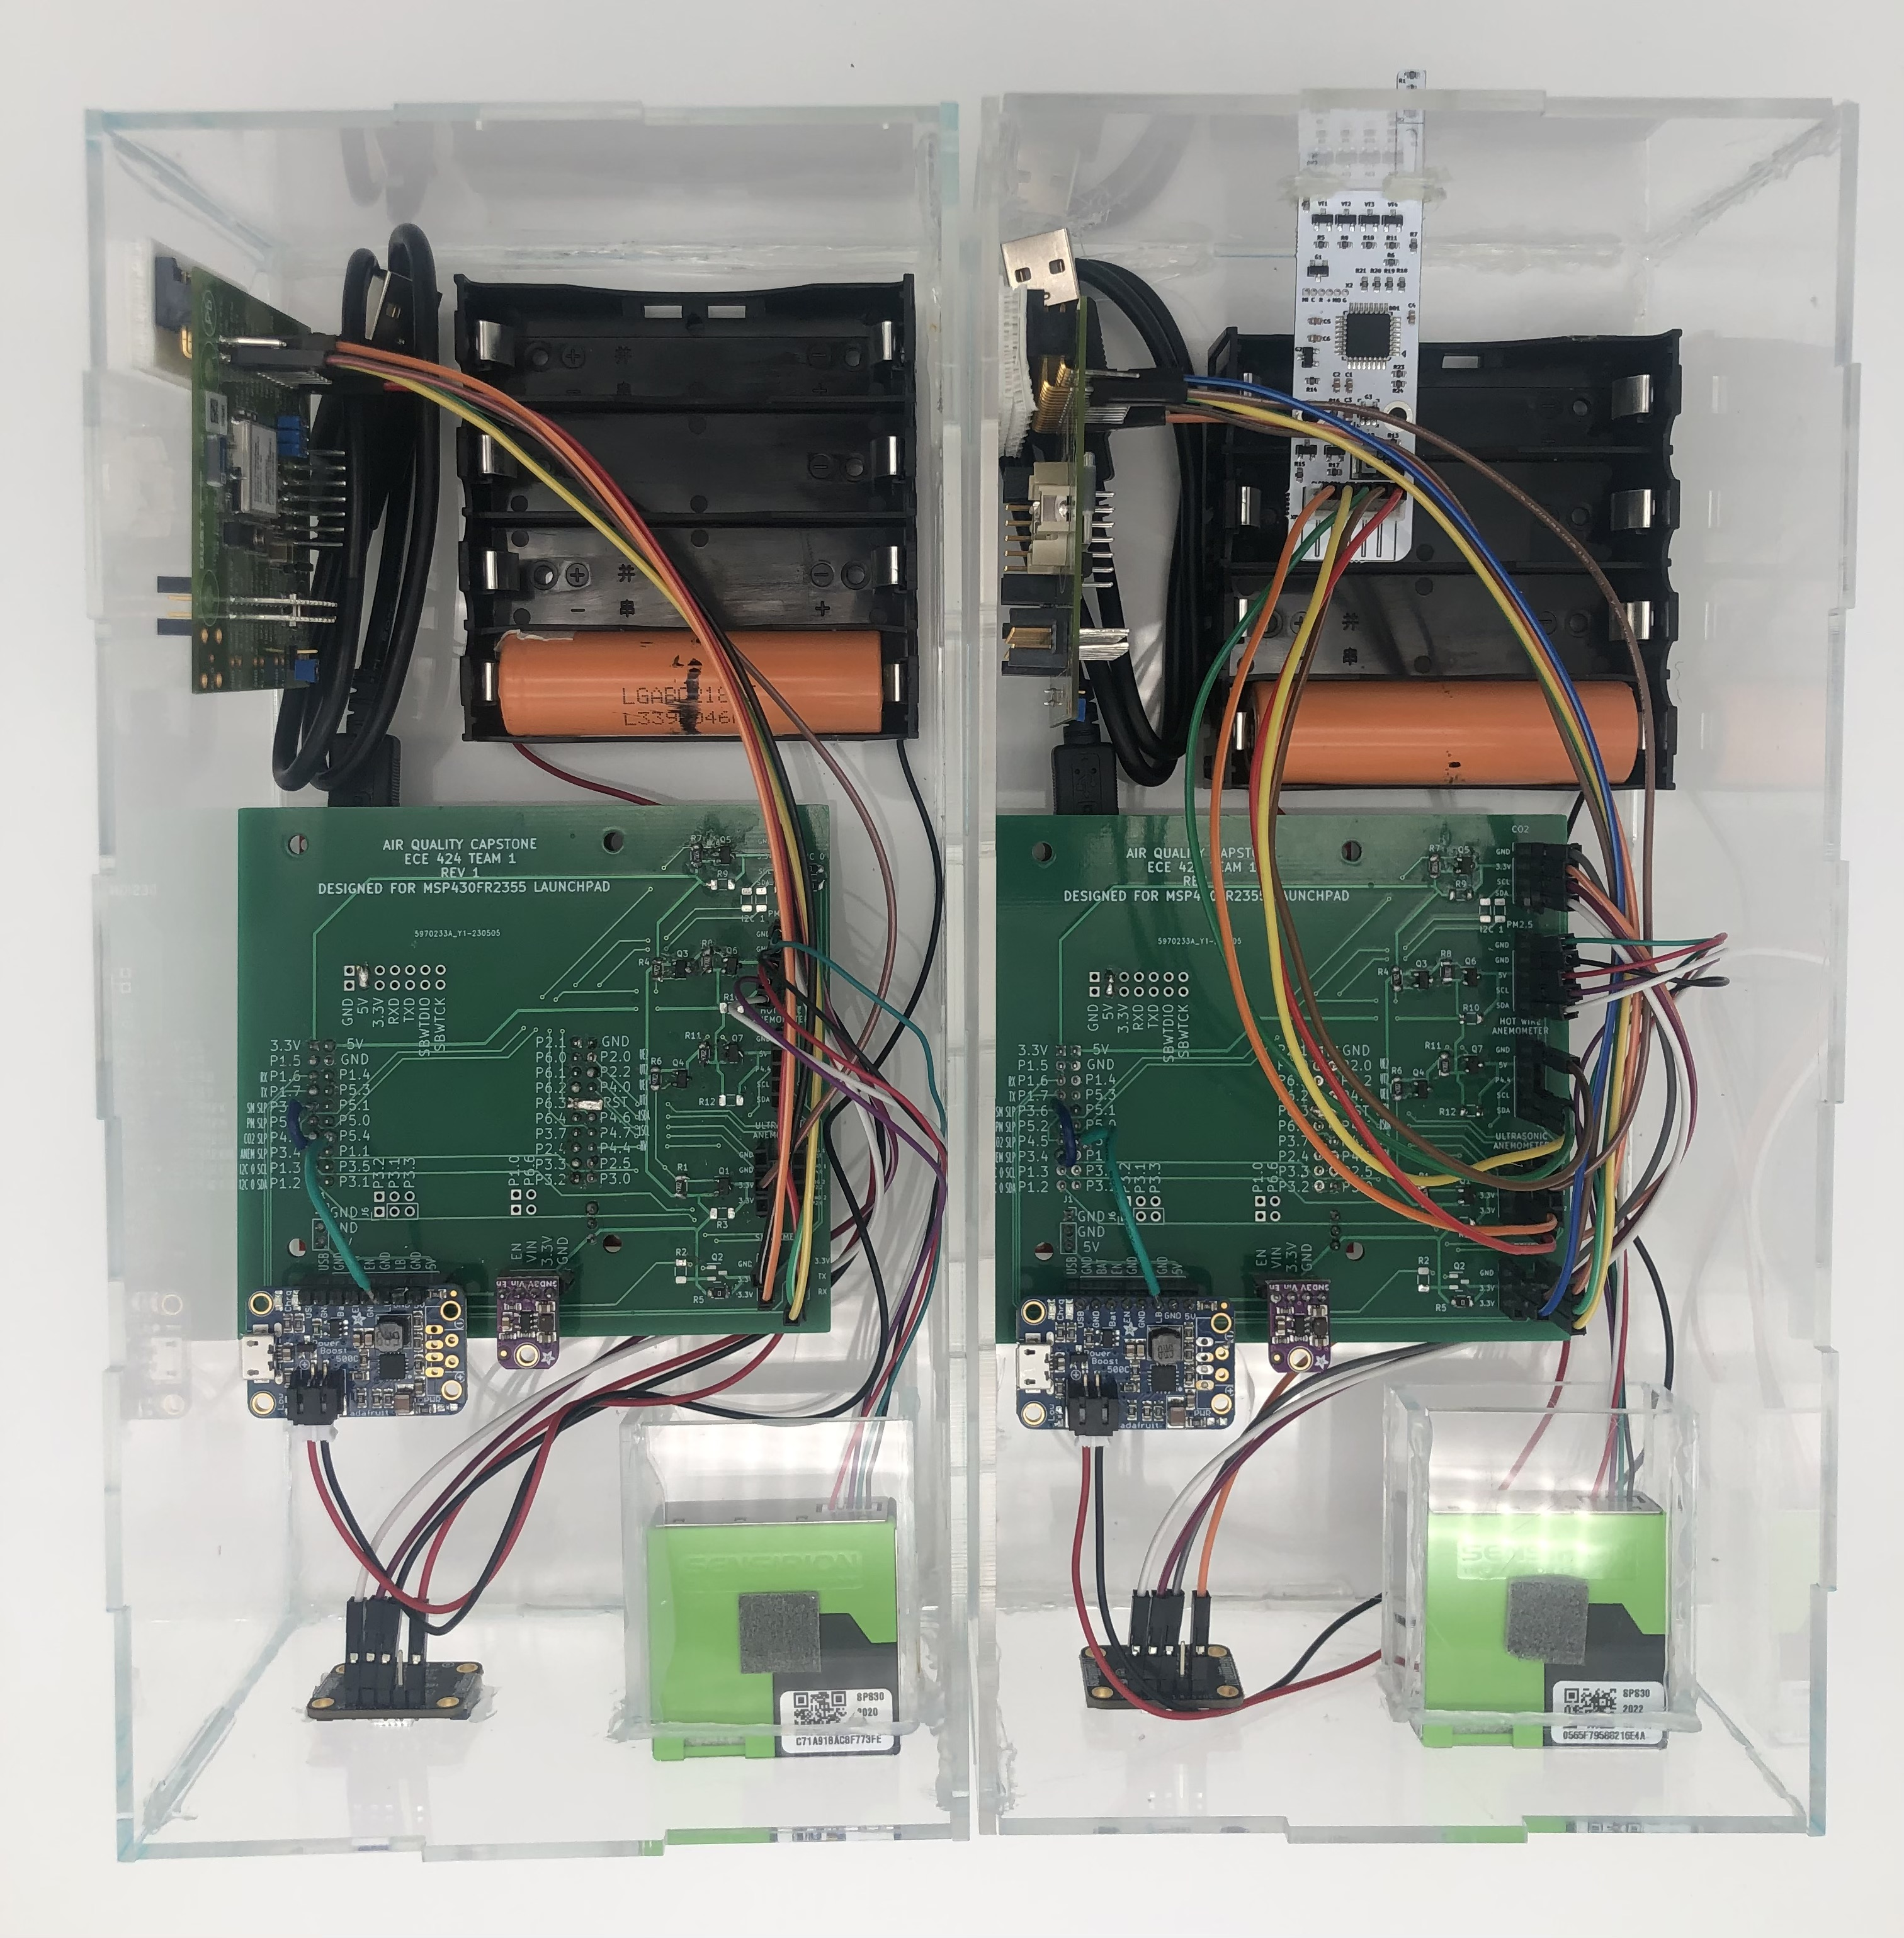
\includegraphics[width=0.8\textwidth]{Pictures/topview.jpg}
    \caption[Top view of the node]{Top view of the nodes} 
    \label{fig:results}
\end{figure}
Our project was successful in satisfying all requirements. Our team was able to build 4 working nodes that all communicate using SmartMesh. The CO$_2$ and PM2.5 sensors are working properly within the acrylic enclosure built. The tables below show estimations of how often we can collect and publish data based on how long we want our batteries to last. The captured intervals can be modified using only 1 line in the code for the system. As shown in the power consumption figure, the hot wire anemometer is the most power hungry part of this project. We recommend that teams look into using an alternative option like the ultrasonic anemometer.\\\\
% Please add the following required packages to your document preamble:
% \usepackage{graphicx}
\begin{table}[h]
\centering
\resizebox{\textwidth}{!}{%
\begin{tabular}{|l|l|l|l|}
\hline
Sensor & 3 Months Battery Life & 6 Months Battery Life & 1 Year Battery Life \\ \hline
CO$_2$  & 8 min 30 sec (510 sec)     & 18 min (1,080 sec)     & 37 (2,220 sec)       \\ \hline
PM2.5  & 16 min (960 sec)      & 34 min (2,040 sec)      & 72 min (4,320 sec)       \\ \hline
\end{tabular}%
}
\caption{Component Measurement Periods for 3 month, 6 month, and 1 year battery life for units without anemometer
}
\label{tab:no annemometer}
\end{table}

% Please add the following required packages to your document preamble:
% \usepackage{graphicx}
\begin{table}[htbp]
\centering
\resizebox{\textwidth}{!}{%
\begin{tabular}{|l|l|l|l|}
\hline
Sensor             & 3 Months Battery Life & 6 Months Battery Life & 1 Year Battery Life \\ \hline
CO$_2$             & 27 min (1,620 sec)     & 61 min (3,660 sec)     & 170 min (10,200 sec) \\ \hline
PM2.5              & 32 min (1,920 sec)     & 72 min (4,320 sec)    & 195 min (11,700 sec) \\ \hline
Hotwire Anemometer & 14 min 38 sec (878 sec)      & 33 min (1,980 sec)     & 90 min 50 sec (5,450 sec)   \\ \hline
\end{tabular}%
}
\caption{Component Measurement Periods for 3 month, 6 month, and 1 year battery life for units with a hot wire anemometer
}
\label{tab:hot annemometer}
\end{table}

% Please add the following required packages to your document preamble:
% \usepackage{graphicx}
\begin{table}[htbp]
\centering
\resizebox{\textwidth}{!}{%
\begin{tabular}{|l|l|l|l|}
\hline
Sensor                & 3 Months Battery Life & 6 Months Battery Life & 1 Year Battery Life \\ \hline
CO$_2$                & 12 min (720 sec)      & 25 min (1,500 sec)     & 51 (3,060 sec)       \\ \hline
PM2.5                 & 22 min (1,320 sec)     & 48 min (2,880 sec)     & 105 min (6,330) sec  \\ \hline
Ultrasonic Anemometer & 10 sec                & 20 sec                & 40 sec              \\ \hline
\end{tabular}%
}
\caption{Component Measurement Periods for 3 month, 6 month, and 1 year battery life for units with an ultrasonic anemometer
}
\label{tab:no annemometer}
\end{table}
% Please add the following required packages to your document preamble:
% \usepackage{graphicx}
\begin{table}[htbp]
\centering
\resizebox{\textwidth}{!}{%
\begin{tabular}{|l|l|l|l|}
\hline
Configuration         & 3 Months Battery Life & 6 Months Battery Life & 1 Year Battery Life \\ \hline
Without Annemometer   & $\sim$820 KB          & $\sim$810 KB          & $\sim$700 KB        \\ \hline
Ultrasonic Anemometer & $\sim$16.15 MB        & $\sim$16.14 MB        & $\sim$16.27 MB      \\ \hline
Hotwire Anemometer    & $\sim$370 KB          & $\sim$334 KB          & $\sim$258 KB        \\ \hline
\end{tabular}%
}
\caption{ Log file sizes after draining batteries for each configuration set to 3 month, 6 month, and 1 year battery life
}
\label{tab:CONFIG OF ALL}
\end{table}